


\chapter{Introduction}


\section{HLS Overview}
\label{sec:hls_view}

This report will talk about high level synthesis (HLS) desing using FPGA. 

Unlike traditional hardware descirption language (VHDL, Verilog), HLS uses high level languages such as \verb|C| and \verb|C++| to design product using FPGA. The advanatage is the speed of learning compared to traditional language.\\


\todo{introduction} \underline{\textit{Introduction}:}

\begin{itemize}

\item \textit{To adapt more the introduction}

\item \textit{Insert references and books}

\end{itemize} 

\subsection{FPGA Benefits and introducing HLS}

FPGA offers some extra benefits, compared to some other computing platform such as multicore CPU and GPU. These are:

\begin{itemize}

\item Reconfiguribilty: the architecture of an FPGA can be adapted depending on the demand of the application

\item Parallelism

\item Less power compared to other platform for the same task

\end{itemize}

However, FPGA was suffering from serious drawback such as:

\begin{itemize}

\item The complexity of hardware language: learning them, and debugging their application

\item Lack of standard libraries to accelerate development

\end{itemize}

This why HLS has comes and introduce the idea of using \tbi{high level languages to design hardware modules}. 

\section{Development Environment and Hardware}

The development environment used is from \verb|Vivado| company, and the baord will be the \verb|Basys3| from \verb|Digilent|.

\newpage
\section{FGPA Concepts}

As stated in \autoref{sec:hls_view}, HLS is about bringing programming concept to the hardware using FPGA. 

In this section, we present a high level overview about the FPGA concept that we should now in order to do some HSL programming. The overview map is presented in \autoref{fig:intro_hls:fpga_concept}

\begin{figure}[h]
\centering
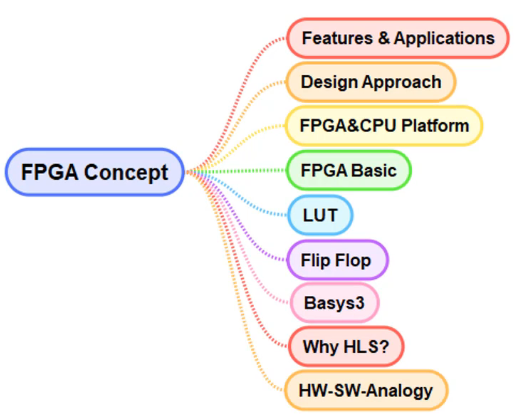
\includegraphics[scale=0.5,frame]{Figures/intro_hls/fpga_concept}
\caption{FPGA Concepts Overview}
\label{fig:intro_hls:fpga_concept}
\end{figure}

\subsection{Design Level}

FPGA desing is categorized in 3 different levels as shown in \autoref{fig:intro_hls:design_types}.

\begin{figure}[h]
\centering
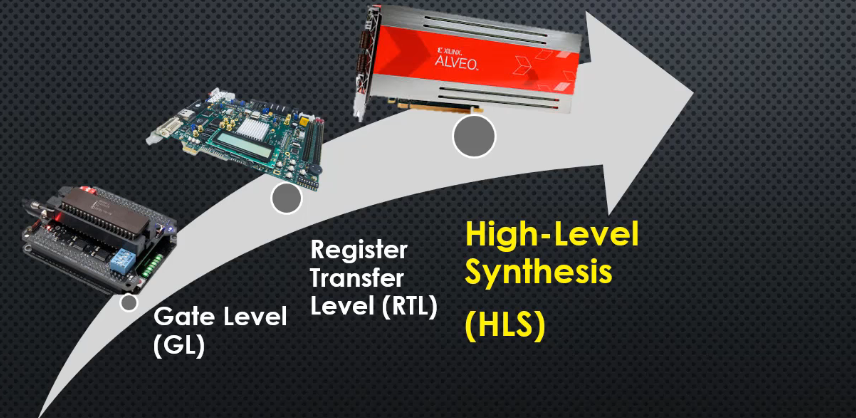
\includegraphics[scale=0.5,frame]{Figures/intro_hls/design_types}
\caption{FPGA Design Levels}
\label{fig:intro_hls:design_types}
\end{figure}

\begin{itemize}

\item Gate Level: using simple gates (AND,OR,$\cdots$). This allow hardware designers to implement small circuits on small FPGPA.

\item RTL: with more advanced in resources and capacity on FPGA, RTL became the fundamental concept in desinging ciruit. RTL main languages are \verb|VHDL| and \verb|Verilog|.

However, these languages are complex because they require deep hardware knowledge, and its very close to the gate level. It is the equivalent of \verb|assembly| in the software world.

\item HLS: it is using \verb|C| and \verb|C++| to map complex algorithm to the hardware, with low knowdlege on the hardware. 

The HLS is not simply a lanuage, but also an optimzation technique and some toolset, which can automatically generate the RTL code for us

\end{itemize}

\todo{Design Level} \underline{\textit{Design Level}:}

\begin{itemize}

\item  \textit{To review and Adapt the design level points later}

\item \textit{see section 2, video 5, part 1}

\end{itemize}

\subsection{FGPA and CPU}

We hilight the differences between CPU and FPGA

\begin{itemize}

\item CPU: a computing platform with fixed architecture, with fixed hardware architecture, controlled by a set of commands or instructions.

\item FPGA: also a computing platform, but with no dedicated architecture.

Using HLS, each \verb|C| or \verb|C++| code has its own optmized hardware architecture, which leads high performance execution of some algorithm using FGPA.

\end{itemize}

\newpage
Also, when CPU tends to translate the programming code into assembly code and executed \textit{sequentialy}, whereas FGPA tools translate the code into a set of hardware block and execut the code in \textit{parallel}. 

\begin{figure}[h]
\centering
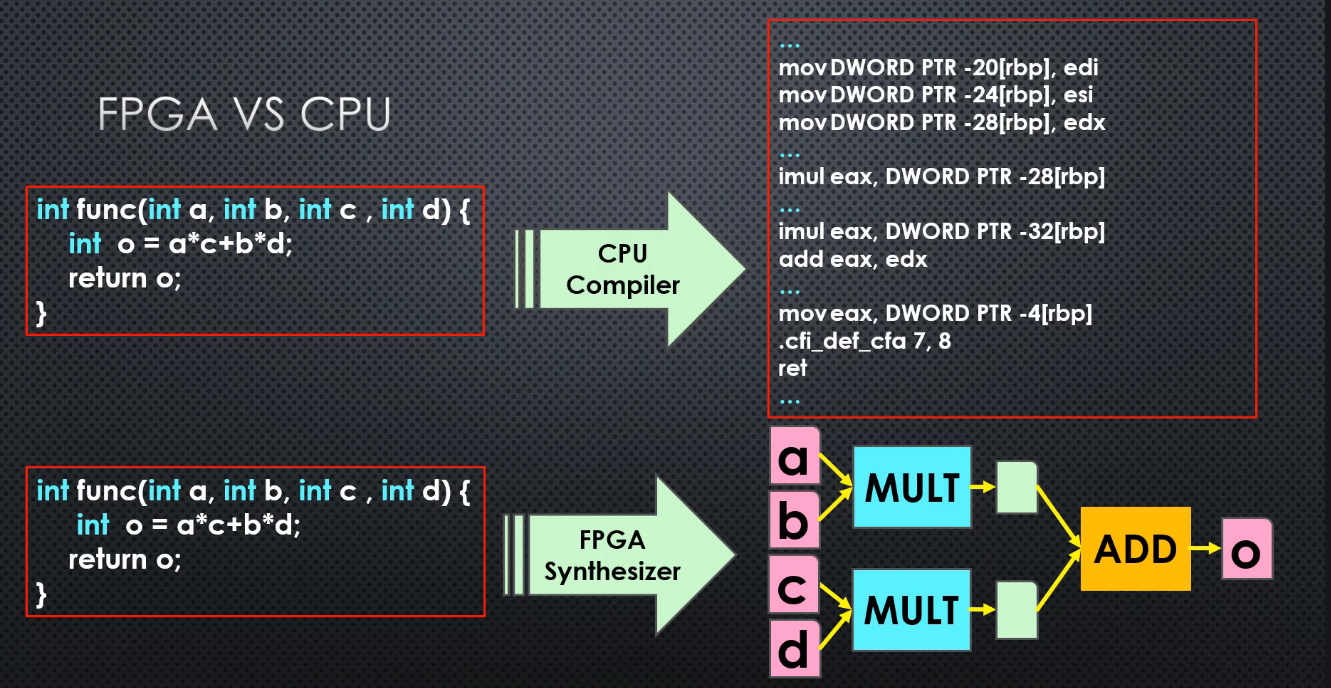
\includegraphics[scale=0.3,frame]{Figures/intro_hls/fgpa_vs_cpu_1}
\caption{FPGA Vs CPU: Sequential vs Parallelism}
\label{fig:intro_hls:fgpa_vs_cpu_1}
\end{figure}

\todo{FGPA vs CPU Parallelism and Sequential} \underline{\textit{FGPA vs CPU Parallelism and Sequential}:}

\begin{itemize}

\item \textit{Source: section 2, video 6, course 1}

\item \textit{To reinsert the picture where we illusrtate adding operation using CPU model (a register and an ALU)}

\item \textit{To read this model from the microcontroller book, how a program is executed on a CPU}

\end{itemize}


\newpage
\subsection{FPGA Structure}

Internal FGPA structure is invisible to the user in HLS programming, but we explore the main components so we can undesrstand later the tools reports.\\

From a concept (or sofware point of view), an FPGA consist of 2 main layer (as shown in \autoref{fig:intro_hls:fgpa_layer}):

\begin{figure}[h]
\centering
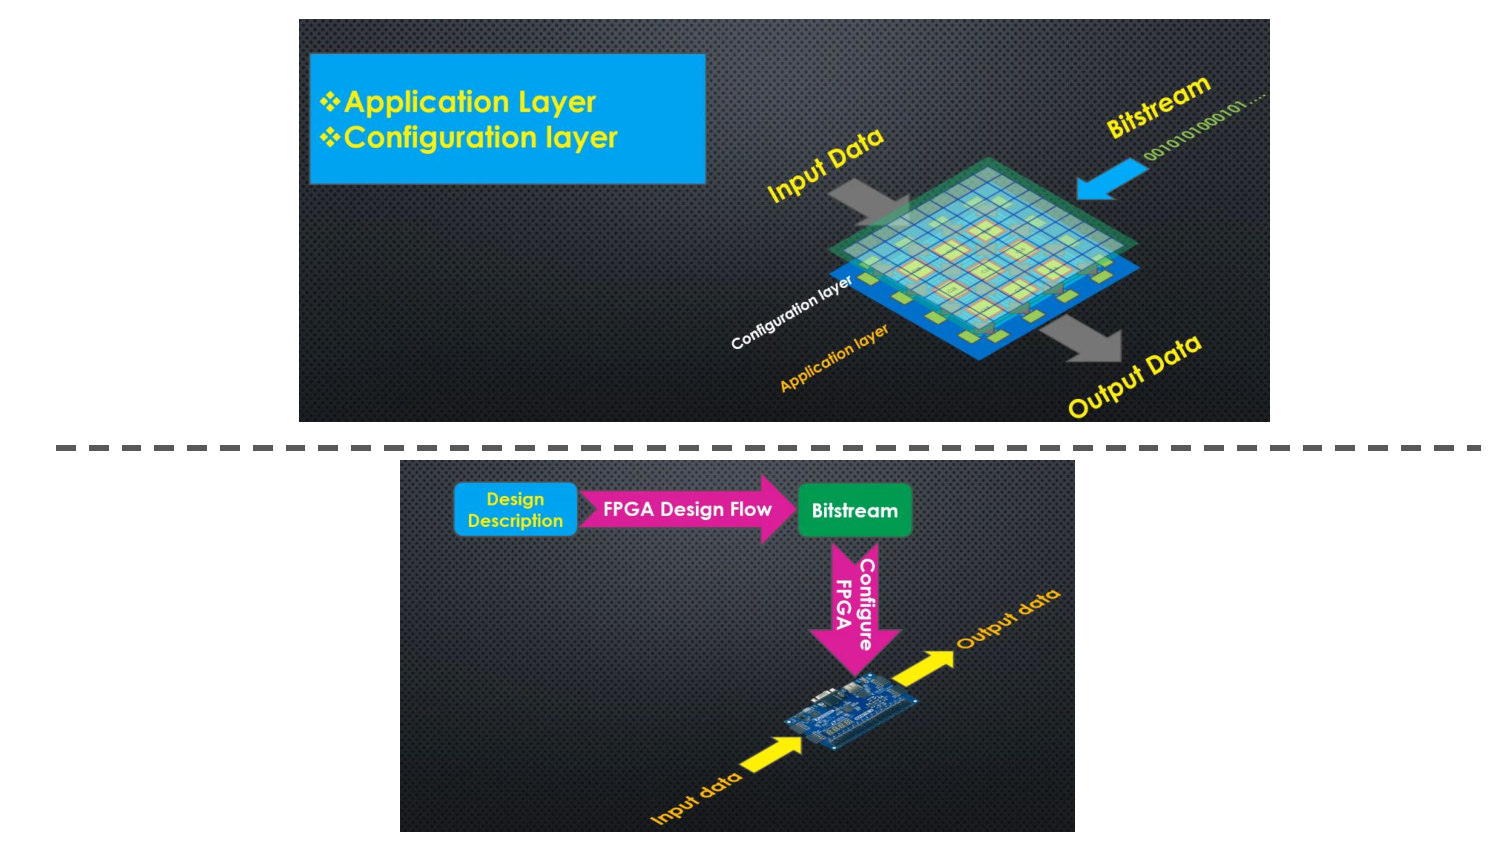
\includegraphics[scale=0.7,frame]{Figures/intro_hls/fgpa_layer}
\caption{FPGA Structure: layer view}
\label{fig:intro_hls:fgpa_layer}
\end{figure}


\begin{enumerate}

\item Application layer: contains all the hardware module to implement some algorithm

Once this layer is configured we can apply the input data to obtain some output

\item Configuration layer: consist of memory cells to configure the application layer.

The configuration data saved in this module is called \textit{bit stream}, and it is generated by systhesis tools.

\end{enumerate}

The role of sotware design suit is to transform the description language into bitstread, then use this bistream to impelemment some circuit using the FPGA, as shown in $\mathrm{2}^\mathrm{nd}$ picture of \autoref{fig:intro_hls:fgpa_layer}\\

\todo{synthesis tool and bitstream} \underline{\textit{synthesis tool and bitstream}:} \textit{To review later this idea after doing some applications}.\\

\newpage
Now from a physical side, an FGPA composition is shown in \autoref{fig:intro_hls:fgpa_composition}.

\begin{figure}[h]
\centering
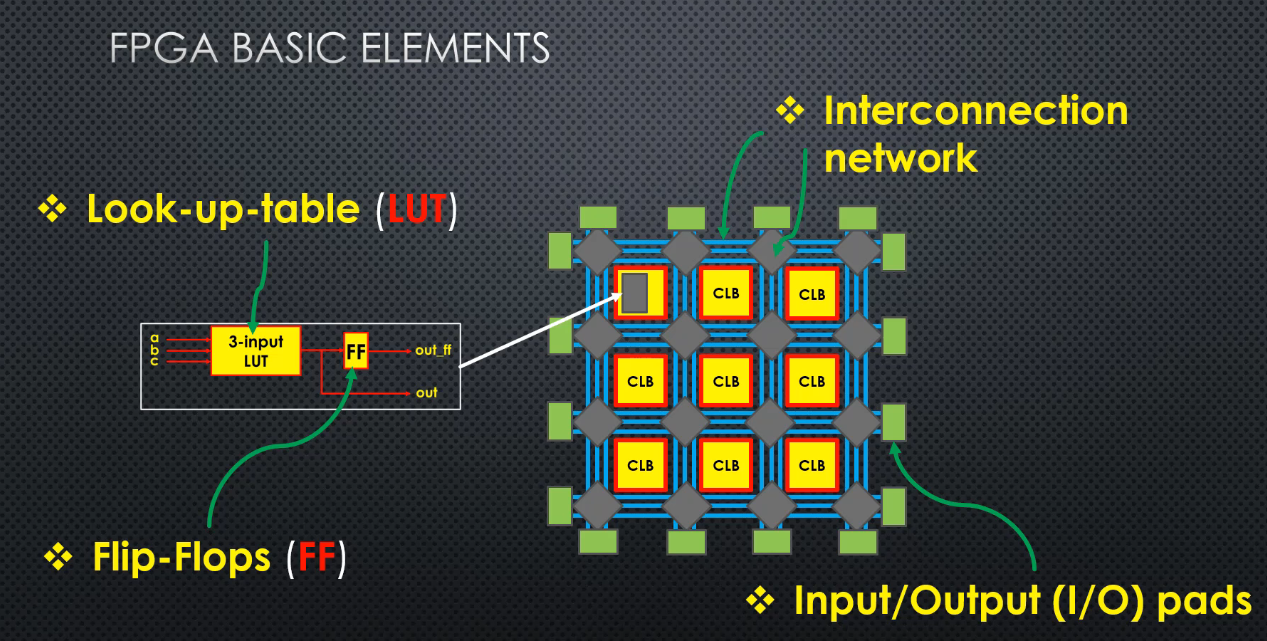
\includegraphics[scale=0.35,frame]{Figures/intro_hls/fgpa_composition}
\caption{FPGA Structure: pyhsical composition}
\label{fig:intro_hls:fgpa_composition}
\end{figure}

\begin{itemize}

\item A look up table (LUT): to implement some logic function

\item A flip flop: a register which saves the output of LUT

\item IO ports: for data manipulation

\item Interconnection network: to connect different resources of FGPA

\end{itemize}

\newpage
\subsection{Look Up Table}

A LUT keeps the output of some logic function for all the input combinations. Examples are shown in \autoref{fig:intro_hls:LUT_example}

\begin{figure}[h]
\centering
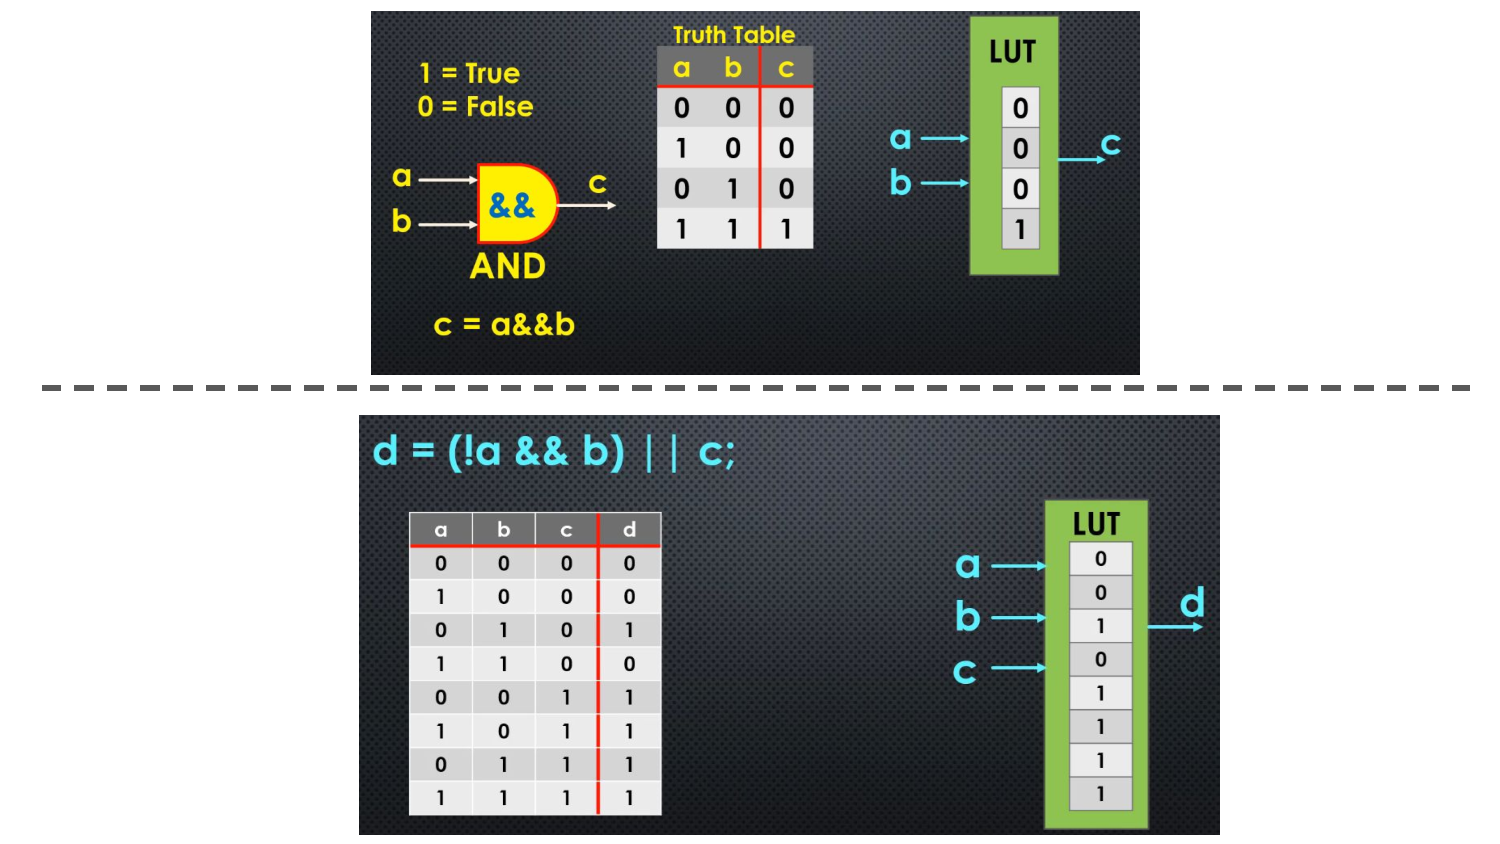
\includegraphics[scale=0.7,frame]{Figures/intro_hls/LUT_example}
\caption{LUT Examples}
\label{fig:intro_hls:LUT_example}
\end{figure}

\begin{itemize}

\item For a basice \verb|AND| gate, a LUT needs only 2 input to track down different output

\item For $\mathrm{2}^\mathrm{nd}$ example, we have 3 inputs leading to 8 outputs. The LUT need 3 inputs to track down the output.


\end{itemize}

\subsection{LUT in FPGA}

Now in FPGA, a LUT has a configuration memory that keeps all the possible outputs of a logic function.

It also has a set of inputs to select the proper cell in the memory corresponding to the inputs logic.

\todo{LUT in FGPA} \underline{\textit{LUT in FGPA}:}

\begin{itemize}

\item \textit{Source: course 1, section 2, video 8}

\item \textit{To redo the writing later}


\item \textit{Main idea}

	\begin{itemize}
	\item \textit{A LUT in FGPA uses multiplexer circuite to select the propoer output nedded, depending on the selections line of the MUX circuit}
	
	\item \textit{Write down the idea of MUX later}	
	
	\end{itemize}


\end{itemize}

\subsection{Flip Flop}
 
In addition to LUT, an FGPA consist also of flip flop, which is a register which can \text{save output} into memory. By having flip flop, we can implement design which depends also on the \textit{past history}, and not only of the present states of the input as in pure combinational logic. 

\newpage 
\section{FPGA Example} 
 
\underline{Main idea:} 
 
\begin{itemize}

\item An FPGA is consisting of \tbi{many slices} 

\item Each slice consist of LUT, flip flop and some basic logic gates

\end{itemize} 

\autoref{fig:intro_hls:fpga_example} present a slice in Xilinx 7-series, which is one of the most common Xilinx FPGA families. 
 
\begin{figure}[h]
\centering
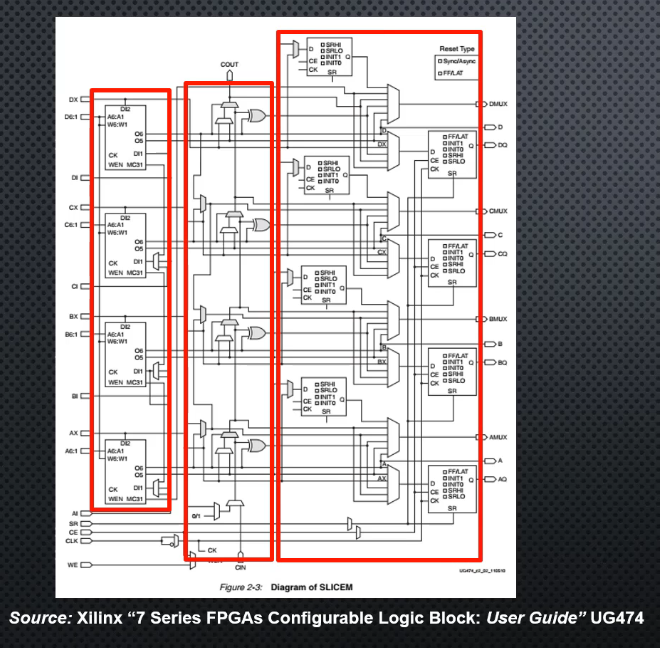
\includegraphics[scale=0.7,frame]{Figures/intro_hls/fpga_example}
\caption{FPGA Slice Example}
\label{fig:intro_hls:fpga_example}
\end{figure}
 
\newpage 
It has three layers of elements:
 
\begin{enumerate}

\item 6 LUT

\item An arithmetic logic cicruit

\item Flilp flop

\item A MUX

\end{enumerate} 
 
Now a \tbi{set of 2 slices and a switch matrix} to connect the slices to the routing on the FPGA is called a \tbi{configurable logic block} or \tbi{CLB}  for short. \tbi{An FPGA} can be considered \tbi{as a 2D array of CLBs} as shown in \autoref{fig:intro_hls:2d_CLB}.

\begin{figure}[h]
\centering
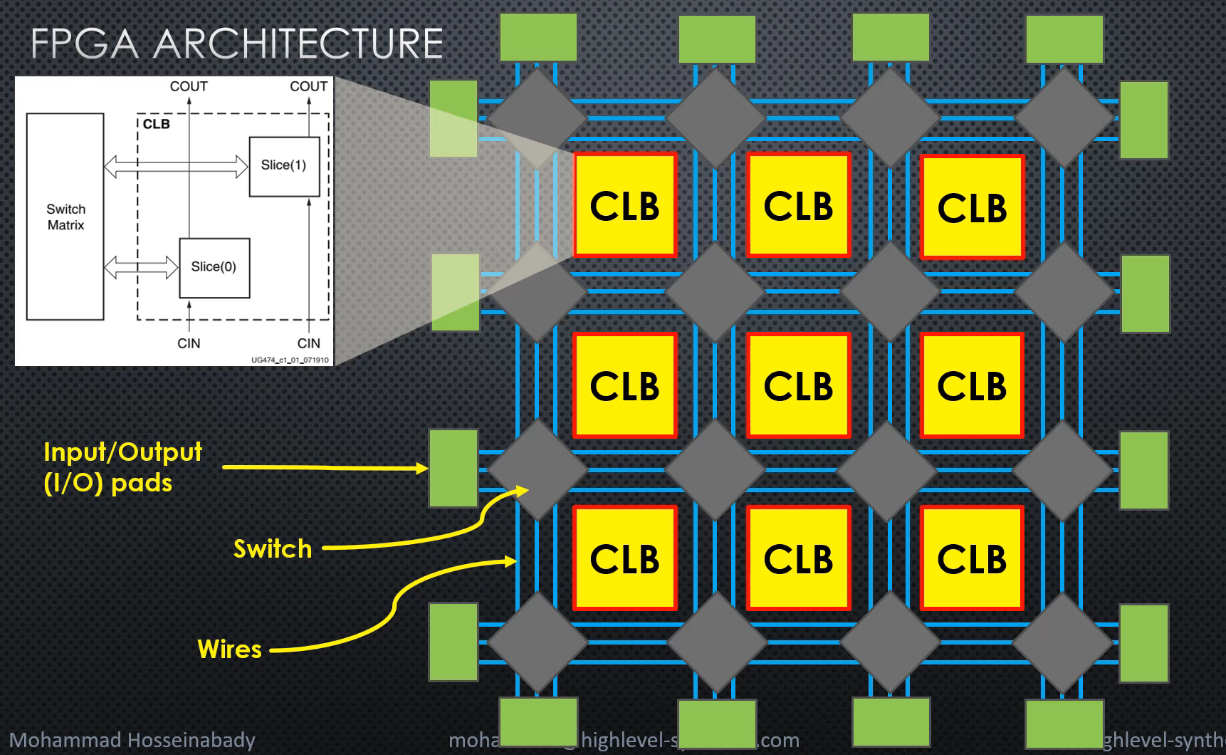
\includegraphics[scale=0.35,frame]{Figures/intro_hls/2d_CLB}
\caption{FPGA as a 2D array of CLB}
\label{fig:intro_hls:2d_CLB}
\end{figure} 

Different CLB are connected through switches and wires to form different complex logic circuit.\\

Now an to a better efficient circuit to impement complex algorithm, an modern FGPA structure \tbi{comes with different additional elements} such as:

\begin{itemize}

\item Block RAM (BRAM) to save large amount of data

\item PLL for driving fgpa at different clock rate

\item High speed serial transeivers

\item Multiply and Accumulate DSP block

\end{itemize}

The FGPA ship along with these extra elements form an development board. The Basys 3 development board will be explored next in \ref{sec:Basys3_board}.

\section{Basys 3 Board Anatomy}
\label{sec:Basys3_board}

\autoref{fig:intro_hls:basys3_board} presents Basys 3 development board, which we will use throughout our development HLS software.

\begin{figure}[h]
\centering
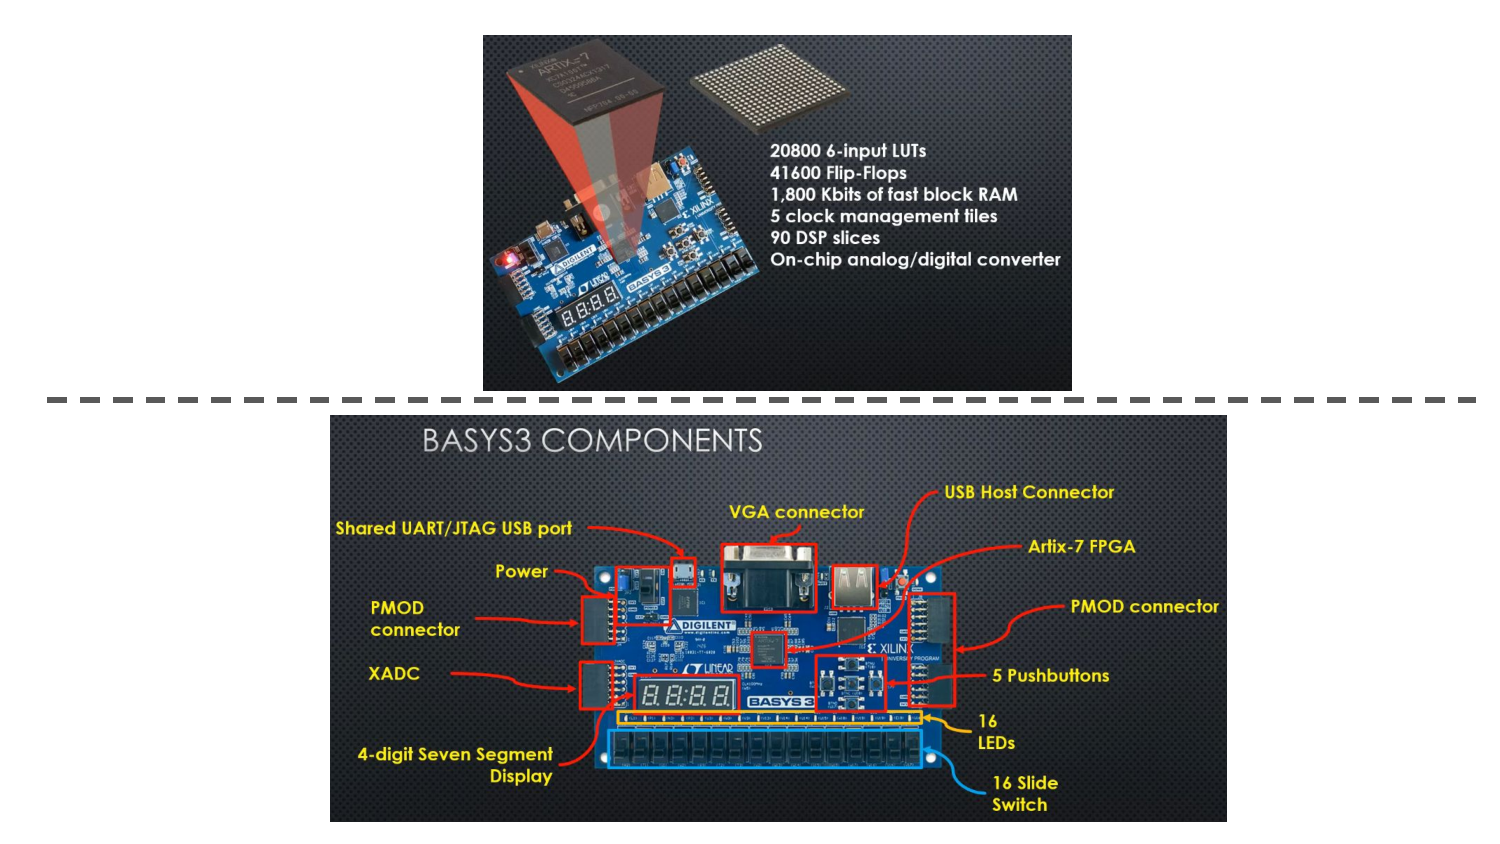
\includegraphics[scale=0.7,frame]{Figures/intro_hls/basys3_board}
\caption{Basys 3 board}
\label{fig:intro_hls:basys3_board}
\end{figure} 

\begin{itemize}

\item The LED are arranged in a common cathode structure

\item The LED of the board are connected to a 330 ohm resistors to prevent damage in case of short circuits

\end{itemize}

\underline{\textit{cathod and anode}:} \todo{cathod and anode}

\begin{itemize}

\item \textit{To review these concepts later, and insert them into an appendix}

\end{itemize}

\newpage
\subsection{Power Source}

\autoref{fig:intro_hls:basys3_power} present the power circuit for the fpga.


\begin{figure}[h]
\centering
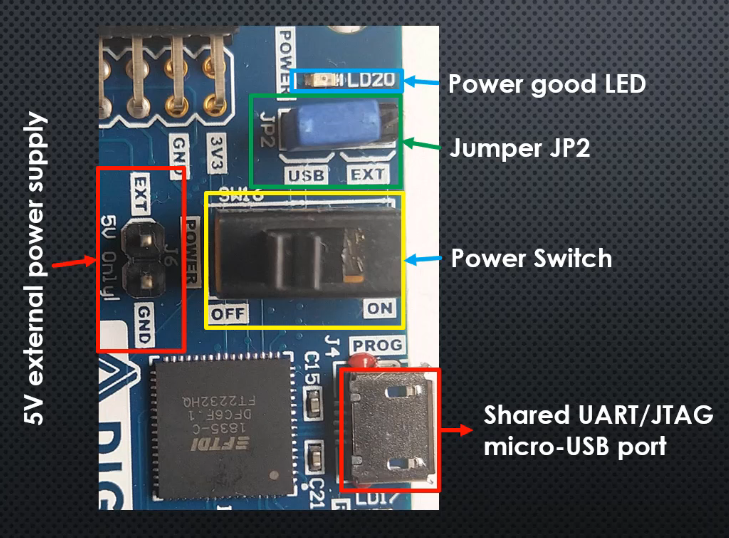
\includegraphics[scale=0.5,frame]{Figures/intro_hls/basys3_power}
\caption{Basys 3 power circuit}
\label{fig:intro_hls:basys3_power}
\end{figure}

The board can take power either from shared UART/JTAG port, or from 5v external board. A jumper j2 is used to select which source we choose, and a power switch can be used to turn on or off the board. The \verb|LD20| Led is used to indicate if power is at normal state throughout the board.


\newpage
\subsection{FPGA Configuration}

After powering up the FPGA, it must be configured. We have 3 modes for configuration as shown in \autoref{fig:intro_hls:fpga_config}.

\begin{figure}[h]
\centering
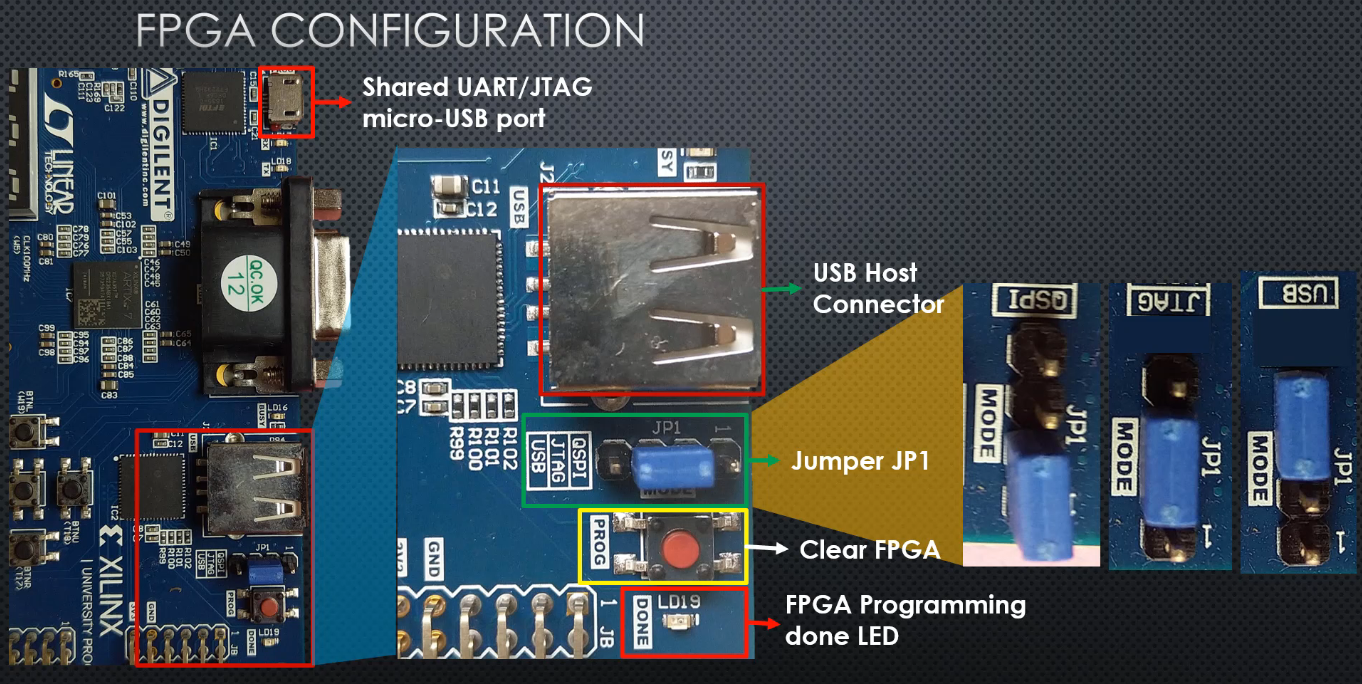
\includegraphics[scale=0.35,frame]{Figures/intro_hls/fpga_config}
\caption{Configuration Modes}
\label{fig:intro_hls:fpga_config}
\end{figure}


\begin{enumerate}

\item Through the shared JTAG usb port

\item Using a file from a usb connector

\item Using the SPI board

\end{enumerate}

\underline{\textit{FPGA configuration}:} \todo{FPGA configuration}

\begin{itemize}

\item \textit{Source: course 1, seciton 2, video 10}

\item \textit{To review this section later after doing some examples}

\end{itemize}

Once the programming done, the \verb|LD19| will be on to indicate firmware flashing has been done.
 
\newpage
\section{Hardware Software Analogy}

Since we will desing hardware modules using software, it is a good idea to establish some analaogy between software and hardware. This help us to have hardware description in the eyes of software.

The analogy between hardware modules and high level langugae contians some similiarities and also some differences.\\


\autoref{similarities_soft_hard} present the similarities between standard \verb|C| function and some hardware module to impelement.

\begin{figure}[h]
\centering
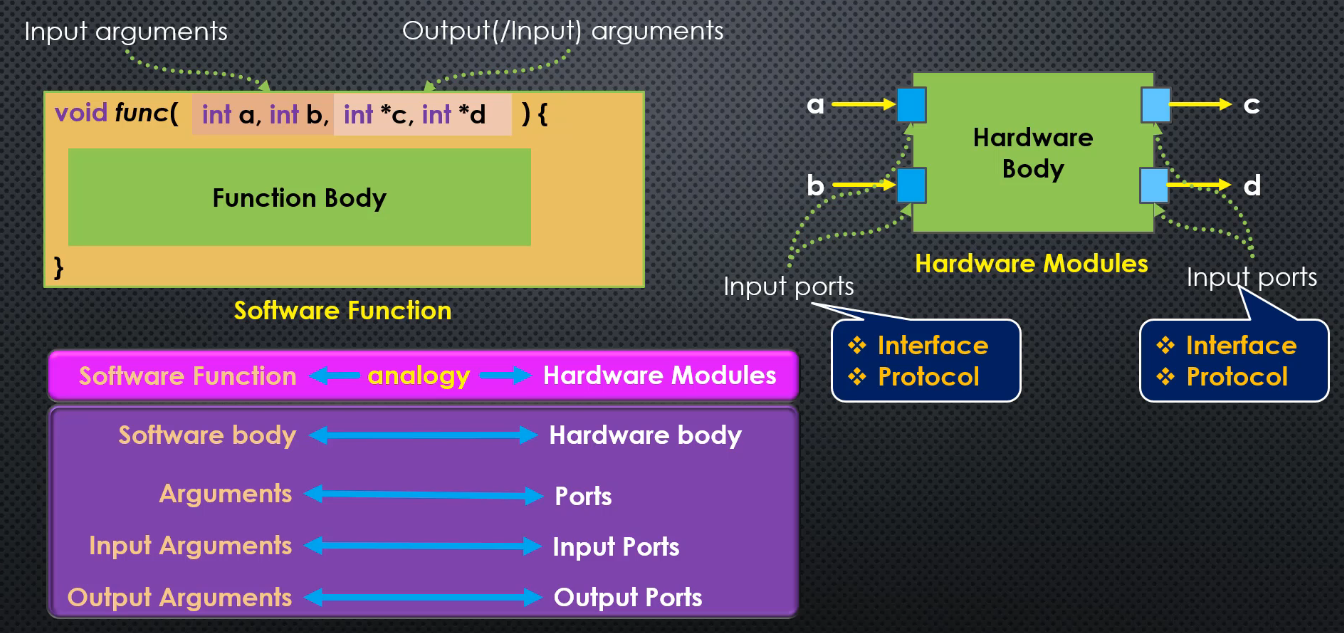
\includegraphics[scale=0.35,frame]{Figures/intro_hls/similarities_soft_hard}
\caption{Similarities between software and hardware}
\label{fig:intro_hls:similarities_soft_hard}
\end{figure}

\autoref{fig:intro_hls:differences_soft_hard} present the differnces

\begin{figure}[h]
\centering
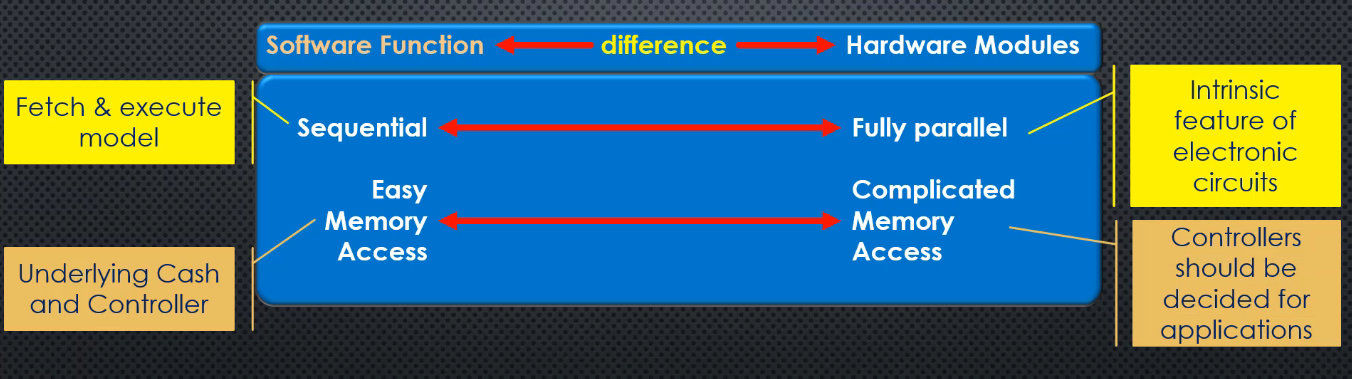
\includegraphics[scale=0.35,frame]{Figures/intro_hls/differences_soft_hard}
\caption{Differences between software and hardware}
\label{fig:intro_hls:differences_soft_hard}
\end{figure}

Now the take away is that HLS hide these details (these differences) through compiler directives using pragma, which guide synthesis tool to add these differences.\\

\newpage
\underline{\textit{Soft Hard differences}:} \todo{Soft Hard differences}

\begin{itemize}

\item \textit{Source: course 2, section 2,  video 12}

\item \textit{This is a very important topic}

\item \textit{To review the memory model inside a traditional cpu, the fetch exectue model, once I finishi this course, and the course of microcontroller drivers}

	\begin{itemize}
	\item \textit{Also once finished with this, to see how the 		memory model interact in FPGA, the protocol idea and 				implemeting an interface, I didn't quiet understood them yet}

	\item \textit{I quote: However, ports in a hardware module should implement a specific interface with the associated protocols to access a memory cell or communicate with other modules}.
	
	\end{itemize}
	
\end{itemize}

\newpage
\section{Environment Setup}

\uti{Vivado Steps} \todo{Vivado Steps}

\begin{itemize}

\item \textit{Source: section 3, video 13 and 14}

\item \textit{Talk about different stages of design, from C programming, simulation for debuggign, types of simulation,$\cdots$}

\item \textit{To much details for now, I will get back to it once I understand more and do some concrete examples}


\end{itemize}








